\documentclass{article}
\usepackage[a4paper, total={7in, 9in}]{geometry}
%\usepackage[KOI8-R]{inputenc}
%\usepackage{cmap}
%\usepackage[T2A]{fontenc}
\usepackage[english]{babel}
\usepackage{verbatim}
\usepackage{array}
\usepackage{cancel}
\usepackage{amssymb}
\usepackage{amsfonts}
\usepackage{amsmath}
\usepackage{amsthm}
\usepackage{amscd}
\usepackage[dvips]{graphicx}
\usepackage{color,colortbl}
%\usepackage{makeidx}
\usepackage{multirow} 
\usepackage{longtable}
%\usepackage{xfrac}
\usepackage{url}
\usepackage{rotating}

\usepackage{framed} 

\definecolor{gray}{rgb}{0.8,0.8,0.8}
\definecolor{ltgray}{rgb}{0.9,0.9,0.9}
\definecolor{darkgray}{rgb}{0.6,0.6,0.6}
\definecolor{Gray1}{gray}{.8}
\definecolor{shadecolor}{gray}{0.9}  
\newcommand{\tw}{\textwidth}
\newcommand{\red}{\textcolor{red}}
\newcommand{\green}{\textcolor{green}}
\newcommand{\blue}{\textcolor{blue}}
\newcommand{\gray}{\textcolor{gray}}

%=============================================================================
\newcommand{\prm}[1]{\texttt{\textbf{{#1}}}}
\newcommand{\pr}[1]{\texttt{{#1}}}
\newcommand{\sg}{$StereoGene$\ }
\newcommand{\sgv}{$StereoGene$ version 2.50\ }

\usepackage{ifthen}
\newcounter{rowc}

\newcommand{\cw}{3.5cm}
\newcommand{\rcf}[1] {\begin{minipage}{\cw}{\prm{#1}}\end{minipage} \setcounter{rowc}{1} }
\newcommand{\rc}[1]
 {\ifthenelse{\isodd{\value{rowc}}}
 {\\ \rowcolor{ltgray} }
 {\\}
 \begin{minipage}{\cw}\prm{#1}\end{minipage}
\stepcounter{rowc}
}
\renewcommand{\arraystretch}{1.2}

%=============================================================================
\title {\sgv}
\author{User manual}

\begin{document}
\maketitle 

\tableofcontents

\section{Introduction}

High-throughput sequencing methods generate massive amounts of data.  The most common first step in interpreting these data is to map the data to genomic intervals and then overlap them with genomic annotations. A major interest in computational genomics is spatial, genome-wide correlation between genomic features (e.g., between transcription and histone modification). The key hypothesis here is that features that are similarly distributed along a genome may be functionally related.

Here we propose the \sg method, which rapidly estimates the genome-wide correlation of two genomic annotations. The method allows correlation of continuous data, eliminating the data loss that occurs when reducing to intervals. To incorporate the analysis of non-overlapping but spatially related features, we use kernel correlation.  Another novel and powerful feature of our approach is the output of local correlation traces that allow overlapping with other correlations (correlation of correlations). 
\subsection{Software availability}
The \sgv C++ source code, program documentation, Galaxy integration scripts and examples are available on the  github repository \url{https://github.com/favorov/stereogene}.

The repository includes four folders: 
\begin{itemize}
\item src is the source folder
\item www contains a fresh copy of the project web page
\item galaxy contains the stub files for Galaxy (https://galaxyproject.org/) integration
\item example is a set of files for a minimalistic run 
\end{itemize}

\subsection{Source code and license}
The software is provided in a form of C++ source code with a makefile for GCC compiler. After cloning or downloading and unpacking the source, say command \prm{<make>} from the shell in the source (\prm{stereogene/src}) folder. 

Our source code is covered by MIT artistic license. We use FFT code by Jens Jorgen Nielsen, its license is shown in the mixfft.c source file.

\subsection{Input and output}
The program reads standard (bed, wigg, etc.) formats for the features to be correlated and a tab-delimited text file with chromosome name and its length pairs on each line as the chromosome length file. The output will be a set of text files. One pair of them (statistics and parameters) is a report that grows line by line with each start of \sg in the current working folder. Others are text files that follow a naming scheme (see below) that allows batch post-processing. On request (using the \prm{plotType} parameter), \sg generates an R script that creates a human-readable report in pdf or html format. If Rscript is not defined PATH (usually in Windows platform) it should be referred in the \prm{Rscript} parameter (for example: \texttt{Rscript="C:/Program Files/R/R-3.6.0/bin/x64/Rscript.exe"})
%========================================================================================
\subsection{Easy start}
\sg has a lot of parameters that change the behavior of the software.  However, all of them have reasonable defaults, actually a run requires two track files and a file with chromosome lengths. The following example is started from the example (\prm{stereogene/example}) folder. First, copy (link) the \sg executable you've biult by \prm{make} in the source folder to the example folder. Then, at a shell prompt, type \vspace{0.5cm}

\begin{center}
\texttt{./StereoGene chrom=chromLength -r H3K4me1.bed H3K4me1.bed}\vspace{0.5cm}
\end{center}

The first parameter refers to the file with the length of the chromosomes, the parameter -r tells the program to generate an R script for visualizing the results, other parameters define the input tracks.

For convinces some parameters can be collected in the configuration file (syntax of this file see below, section \ref{cfg}).
To include the configuration file use parameter \prm{cfg=<config\_file>}.

For more complicated case see Section \ref{case2}.
%==========================================================================================
\subsection{Directory structure}
The program creates many files. To manage the files, the directory structure is recommended. The user can define several directories:\vspace{0.5cm}

%\renewcommand{\arraystretch}{1.2}
\begin{longtable}{p{3.3cm}p{5cm}p{5cm}}
\caption{Directoty structure}\\\hline
Path & Description &\\\hline
\rcf {trackPath=<path>}
	& Path to the input tracks. 
		& The program will search input files here
\rc {profPath=<path>}	
	& Path to profiles
		& directory for temporary binary tracks
\rc {resPath=<path>	}
	& Path to the result files 
		& directory for the results
\rc {report=<path>	}	
	& Path to the report files (pdf, html) \red{relative to the resPath}
		& directory for pdf/html reports\\\hline
\end{longtable}


This directory structure can be defined in the configuration file. Example:\\

\begin{minipage}{0.3\tw}
\begin{shaded} 
	\begin{verbatim}
	trackPath=./Tracks
	profPath=./profiles
	resPath=./res
	report=report
	\end{verbatim}
\end{shaded}
\end{minipage}
%=============================================================================================
\subsection{More complicated case}\label{case2}

The example uses the tracks \{\pr{H3K4me3.bed H3K9ac.bed H3K27ac.bed\}} -- active histone modifications and \{\pr{H3K9me3.bed, H3K27me3.bed\}} -- repressive modifications. We analyze the correlation of each active modification with each repressive modification.
\begin{enumerate}
\item Find the directory (\prm{stereogene/example/example-section-1.6}), it will be the work folder.
\item It has \prm{Tracks} folder and subfolders \pr{Tracks/active, Tracks/repress} for the active tracks and repressive tracks.
\item Download from \url{https://genome.ucsc.edu/cgi-bin/hgTracks?db=hg38&chromInfoPage=} chromosome file. Put file with chromosomes \pr{chr\_len\_hg38.tab} to working directory
\item Create the configuration file \pr{stereogene.cfg}:

\begin{shaded} 
\begin{verbatim}
chrom=chr_len_hg38.tab          # define the chromosome file
trackPath=Tracks                # define path to the tracks
profPath=profiles               # define path to temporary binary profiles
resPath=res                     # define path to the results
report=report                   # define path to the reports
plotType=pdf                    # define type of the reports
#-------------------------------- define where is the Rscript 
Rscript="C:/Program Files/R/R-3.6.0/bin/x64/Rscript.exe"
\end{verbatim}
\end{shaded}


\item Run \sg: 
\pr{\$./StereoGene active repress}
\item Find and browse the report files \pr{*.pdf} in the directory \pr{res/active/report}
\item Open the file statitics.tsv in Excel or OpenOffice or R and analyse the result
\end{enumerate}

\subsection{How to look at the results}
After running \sg for tracks \prm{ARID2.bgr}, \prm{ARID1B.bgr} (these are proteins from the SWI/SNF complex) with the configuration file:
\begin{shaded} 
\begin{footnotesize}
\begin{verbatim}
chrom=chr_len_hg38.tab
trackPath=../Tracks
profPath=../profiles
resPath=../res
report=report

wSize=1M
bin=200
KernelSigma=3K
crossWidth=30000

plotType=pdf
Rscript="C:/Program Files/R/R-3.6.0/bin/x64/Rscript.exe"
\end{verbatim}
\end{footnotesize}
\end{shaded}
We obtain the pdf result file (Figure \ref{res1}).
\begin{center}
\begin{figure}[!h]
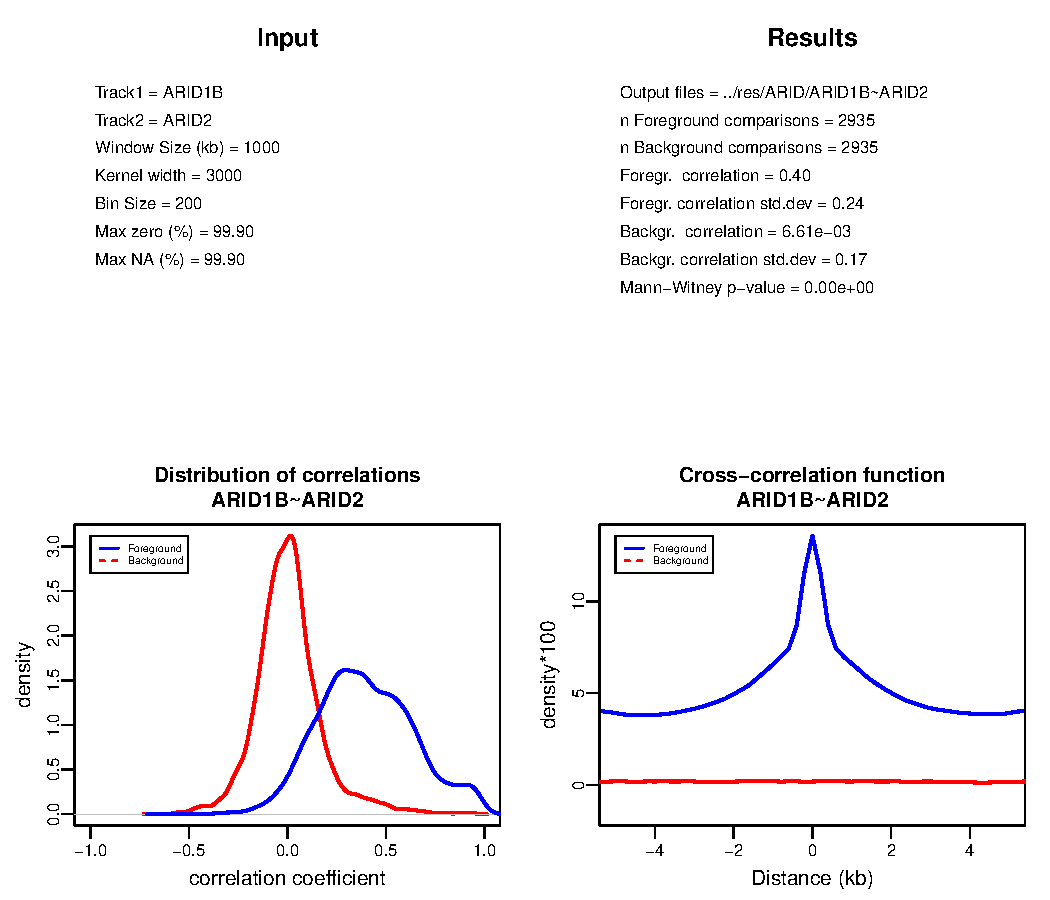
\includegraphics[width=0.75\tw]{fig/ARID1B~ARID2.pdf}
\caption{Result pdf file}\label{res1}
\end{figure}
\end{center}


The upper part of the figure \ref{res1} shows the input track names, the main parameters -- window size and kernel width (left) and the results (right) -- correlation coefficients for the track comparison (foreground) and for the background model. 
The next two plots are shown. The left plot shows the distribution of the correlation for the foreground (blue) and the background (red). The right plot shows the cross-correlations for the foreground and background.

Looking at the plots, it is clear that we observe significant correlations here. Furthermore, the cross-correlation function shows that the dependence of the signals decreases with 1kb distance. This is very good case. 
But sometimes \sg find something like shown on the Figure \ref{res2}

\begin{center}
\begin{figure}[!h]
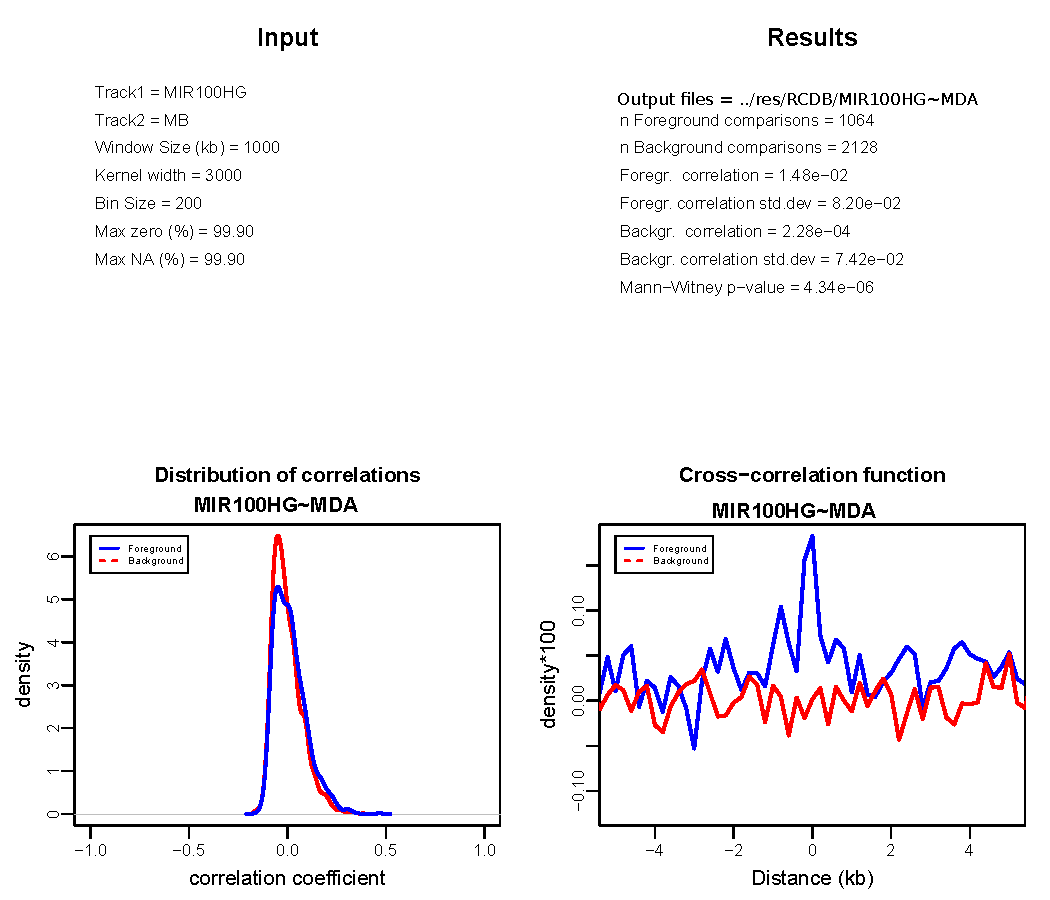
\includegraphics[width=0.75\tw]{fig/mir100~grid_mda.pdf}
\caption{Result pdf file}\label{res2}
\end{figure}
\end{center}

With a very good p-value ($4.3\cdot 10^{-6}$), the correlation is very small ($1.48\cdot 10^{-2}$). The distribution of the correlation coefficients is very close to the background distribution (left plot). The cross correlation plot (right) shows a small peak at zero. We can conclude that we are observing a very small but significant correlation. 
Usually this behavior reflects the fact that the data is sparse.

Another example is shown in the figure \ref{res3}. Here we have a negative correlation, but the cross-correlation function has a sharp drop at zero. This means that two tracks avoid being together.

\begin{center}
\begin{figure}[!h]
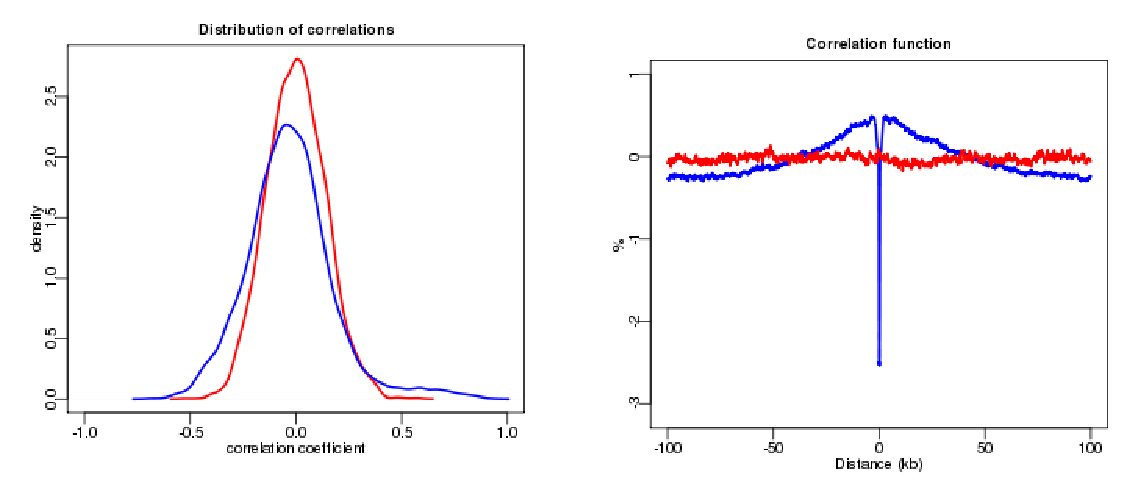
\includegraphics[width=0.75\tw]{fig/corr-ptot3.pdf}
\caption{Result pdf file}\label{res3}
\end{figure}
\end{center}



%============================================================================================================
%============================================================================================================
\section{The calculation workflow}
When started, the software first preprocesses the input data and then performs the requested calculations. The results of the pre-processing steps are stored to save computing time. The next runs of \sg on the same track can reuse the pre-processing results.

%============================================================================================================
\subsection{Preprocessing}
The input is read from the track text file in one of the standard genomic track formats (bed, wig, bedGraph, NarrowPeak, and broadPeak) and then converted into a proprietary binary format file for correlation analysis. The conversion averages all input profiles into small tiling windows (bins) defined by the \prm{bin} parameter. 

The BroadPeak and NarrowPeak formats standard defines a list of possible values for each nucleotide position -- \textit{score}, \textit{signal}, \textit{log-p-value}, and the user can specify which of this Peak data types are to be used (prm{bpType} parameter). 

The program defines the file format using the file name extension:
\begin{table}[!ht]
\caption{Allowed file-name extensions for input tracks}\label{inputFormats}
\begin{tabular}{l|l}
\begin{tabular}{ll}
        \texttt{bed}      	& Bed format\\
        \texttt{wig}      	& Wigg format\\\hline
        \texttt{bedgraph}	&\multirow{4}{*}{Bedgraph format}\\
        \texttt{bed\_graph} &\\
        \texttt{b\_graph}   &\\
        \texttt{bgr}        &\\
        \hline
        \texttt{b\_peak}	&\multirow{4}{*}{Broad Peak format}\\
        \texttt{bpeak}      &\\
        \texttt{broad\_peak}&\\
        \texttt{broadpeak} 	&\\
        \hline
\end{tabular}&
\begin{tabular}{ll}
        \texttt{n\_peak}        &\multirow{4}{*}{Narrow Peak format}\\
        \texttt{npeak}         	&\\
        \texttt{narrow\_peak}	&\\
        \texttt{narrowpeak}    	&\\\hline
        \texttt{model} 			&\multirow{3}{*}{Model file (see Model)}\\
        \texttt{mod}   			&\\
        \texttt{mdl}   			&\\\hline
        \texttt{bigbed}			&\multirow{2}{*}{{\red{\textbf{\large Binary formats do not allowed!}}}}\\
        \texttt{bigwig}			&
\end{tabular}
\end{tabular}
\end{table}

The software allows users to combine several input tracks in a linear combination and use the results of the linear model as one of the tracks used for correlation analysis (see "Model" section).
%============================================================================================================
\subsection{Correlation calculation}
\sg calculates the kerneled correlation, which means that it does not only consider the values of the tracks in the same position, but it integrates all nearby values with weights defined by the kernel. (Figure \ref{kern}).
\begin{figure}[!h]
\begin{tabular}{cc}
\begin{minipage}{0.4\tw}
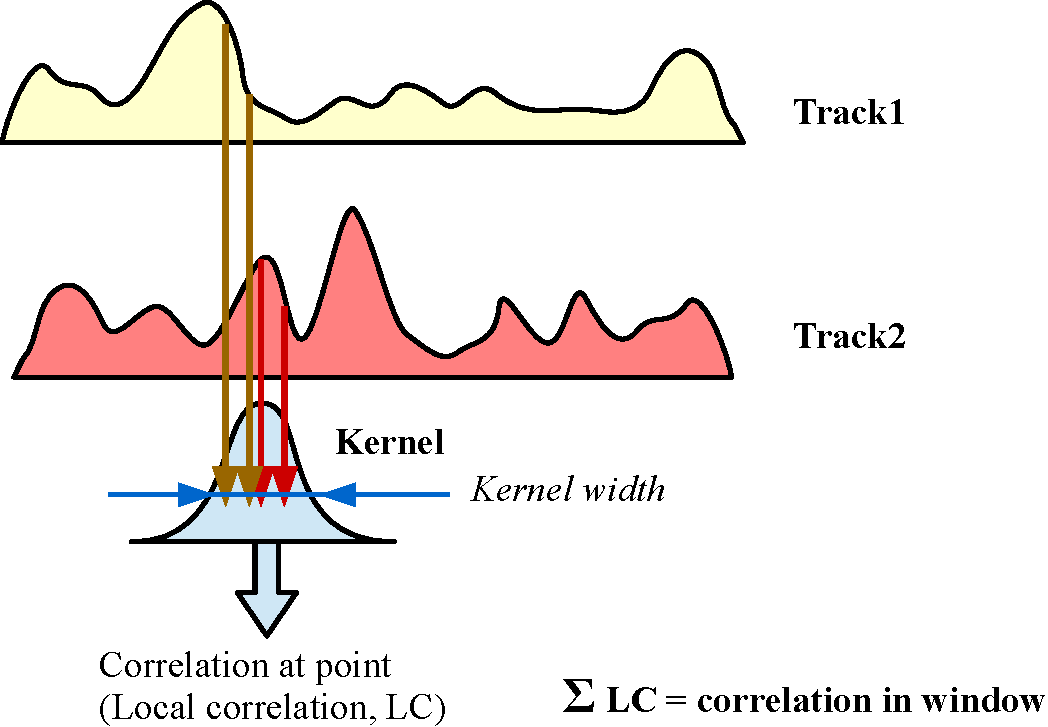
\includegraphics[width=\tw]{fig/kernel.pdf}
\end{minipage}&
\begin{minipage}{0.5\tw}
$$
LC(x)\sim g(x)\int\limits_G \rho(x-t) f(t) dt + f(x) \int\limits_G \rho(x-t) g(t) dt 
$$
$$
corr \sim   \int\limits_{G}\int\limits_{G} \tilde{f}(x)\tilde{g}(y) \rho(x-y) dx dy
$$

\end{minipage}
\end{tabular}
\caption{Kernelled correlation}\label{kern}
\end{figure}



Instead of correlating the whole genome, we compute the correlation of the preprocessed tracks within large windows of fixed size (~1,000,000 bp). The size of these windows is specified by two input parameters (\prm{wSize} and \prm{wStep}). In these parameters, prm{wSize} is the width of the window and \prm{wStep} is the distance between the start coordinates of each window. If \prm{wSize} is equal to \prm{wStep} (default), the windows are tiled and do not overlap. The windows are smaller than whole chromosomes to increase efficiency and to obtain a distribution of values from which to estimate correlation p-values. \prm{wSize} is a technical parameter. If it is too large, there will be too few windows for statistical estimation and the program will be too slow; however, if \prm{wSize} is too small, we will get a very wide variety of local correlation measures instead of a common whole-genome correlation. We recommend using \prm{wSize} = \prm{wStep} = 100k..10M (Figure \ref{sh}A).
\begin{figure}
\begin{tabular}{cc}
\begin{minipage}{0.45\tw}
\textbf{A}
\begin{center}
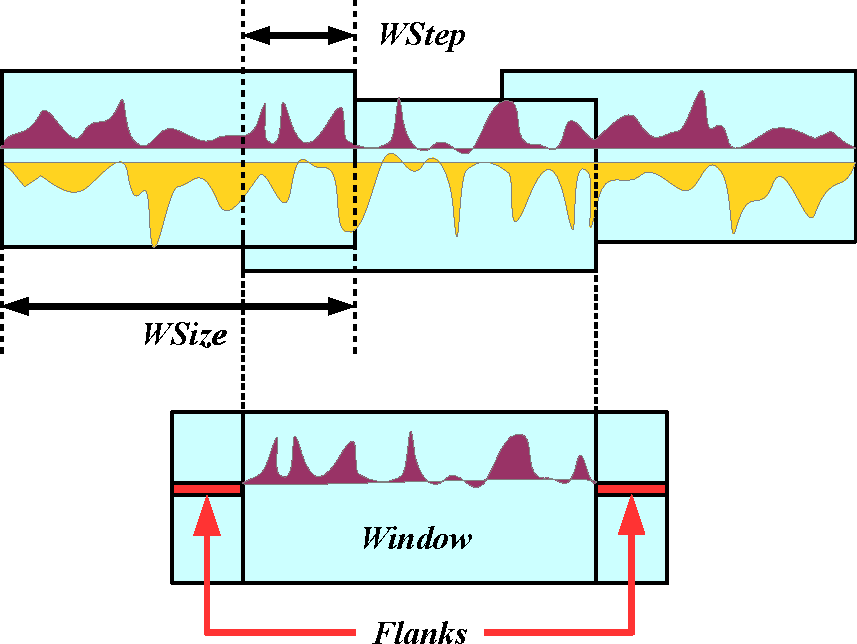
\includegraphics[width=0.9\tw]{fig/window.pdf}
\end{center}
\end{minipage}
&
\begin{minipage}{0.45\tw}
\textbf{B}
\begin{center}
\textbf{Window shuffle}\vspace{0.2cm}\\
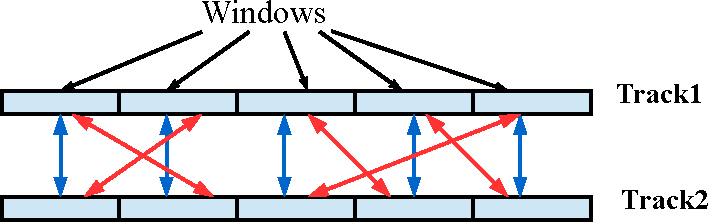
\includegraphics[width=0.9\tw]{fig/wShuffle.pdf}\vspace{0.3cm}\\
\end{center}
\textbf{C}
\begin{center}
\textbf{Local cyclic shuffle}\vspace{0.2cm}\\
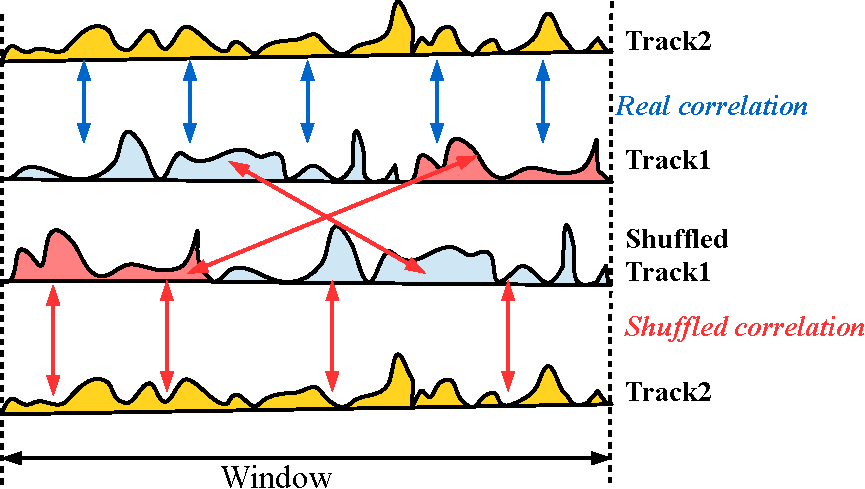
\includegraphics[width=0.9\tw]{fig/LShuffle.pdf}\\
\end{center}
\end{minipage}
\end{tabular}
\caption{Window size and step parameters (A) and shuffling procedure (B,C)}\label{sh}
\end{figure} 

The data on the input tracks is routinely gapped. Some wig files contain zeros. They also contain genomic regions that are not covered by data. There are several ways to interpret this missing data. For example, the coverage of a region could be truly unknown due to a mapping problem. On the other hand, the level could really be 0. Depending on how we interpret the empty areas (NA parameter), we either write zeros in these areas or cover them with random values defined by the \prm{noiseLevel} parameter. The data written to the profile is defined by the formula $x=Norm(e, noiseLevel*sd)$, where Norm - is a random normally distributed value, e, sd - mean and standard deviation of the input data. If the input data is very sparse, the windows containing only 0 or NA values will appear. The correlation in these windows is undefined, so the program ignores them. There are parameters (\prm{maxZero}, \prm{maxNA}, percents) that define which windows should be treated as non-informative.

If the DNA strand is defined (e.g. for genes), the \prm{complFg} parameter indicates whether the information is included in the correlation. The finite size of the windows may cause edge effects; to avoid this, the user can ask the program to add random signal flanks to each window (\prm{flankSize} parameter). However, our experience shows that for large window sizes (e.g., the default 100,000 bp), the flanks have minimal effect on the correlation. 

It is challenging to analytically estimate the null distribution of correlation coefficients that takes into account the dependencies of all features at neighboring positions of the genome. We use a permutation to test the statistical reliability of the result. To do this, we randomly sample pairs of windows, first from one track, then from the other, and evaluate the correlation value for each pair (Figure \ref{sh}B).  The number of sampled pairs is determined by the parameter \prm{nShuffle}. 

Another sparse data approach based on cyclic permutation of non-zero windows. It uses all the features of the standard approach. Instead of comparing different windows, a random cyclic permutation of the tracks is used to compute the background distribution. To use this option, set the parameter \prm{localSuffle}=1. This option is useful for sparse data (Figure \ref{sh}C).

List of calculation parameters shown in the Table \ref{calcPrm}

\begin{longtable}{p{\cw}p{9cm}p{3cm}}
\caption{Calculation parameters}\label{calcPrm}\\
Parameter&Sense&default value\\\hline
\rcf{bin}			&	Bin size. All the tracks are bined with this value.	& 100
\rc{wSize}          &       Window size. Correlation will be done in window.        & 300000 
\rc{wStep}          &       Window step. Windows Shift.                                             & 0 
\rc{noiseLevel}     &       level of the noise to fill NA values                            & 0
\rc{maxZero}                &       Maximum number of zeros in the window (percent)         & 99
\rc{maxNA}          &       Maximum number of NA in the window (percent)            & 99
\rc{complFg = <COLLINEAR | COMPLEMENT | IGNORE\_STRAND>}
	&Flag: \newline
	IGNORE\_STRAND -- ignore strand; \newline
	COLLINEAR -- compare collinear strands;\newline
 	COMPLEMENT -- compare opposed strands. \newline
	If the binary profiles are not separated by strand that works in IGNORE\_STRAND 
		& \prm{IGNORE\_STRAND }
\rc{flankSize}      
	& Size of added flanks (in nucleotides). Necessary to avoid side effects. 
	Recommended value $2\cdot KernelSigma $
		& 0
\rc{KernelSigma} 
	&  Width of the kernel             
		& 1000
\rc{nShuffle}       
	&       Number of shuffle to calculate the background distribution 
		& 10000
\rc{localSuffle}    
	&       Use local shuffle instead of window shuffle 
		&1
\end{longtable}


%============================================================================================================
%============================================================================================================

\section{Input and output}
\subsection{Input}
Here we present the input data in more detail. The basic input file is a track file in one of the formats listed in the table \ref{inputFormats}. 
The program can accept two or more tracks as input. If more than two tracks are defined, all possible track pairs are analyzed (figure \ref{trackPairs}A).

To analyze many tracks, the program can use a batch mode.  
There are two ways of using this option. First, you can define a list of tracks as input (\ref{trackPairs}B,C). Format of the list file -- each line define input track. The filename extension of the list file should be *.list or *.lst. 
Second, you can define the directories as input. In this case, all allowed files in each directory will form a list.

\begin{figure}[!h]
\newcommand{\cor}{Cor}
\begin{tabular}{|l|l|l|}
%======================================
\begin{minipage}{0.22\tw}

\begin{center}
A. 
\end{center}

\begin{tabular}{llll}\hline
&Tr1&Tr2&Tr3\\\hline
Tr1  &\cellcolor{gray}&\cor &\cor \\
Tr2  &\cellcolor{gray}& \cellcolor{gray} &\cor \\
\end{tabular}
\end{minipage}&
%======================================
\begin{minipage}{0.27\tw}
\begin{center}
B.
\end{center}

\begin{tabular}{ll|lll}
&& \multicolumn{3}{c}{list1} \\\hline
&& Tr1&Tr2&Tr3\\\hline
\multirow{2}{*}{\begin{sideways} list1 \end{sideways}}&Tr1&\cellcolor{gray}&\cor &\cor\\
&Tr2&\cellcolor{gray}&\cellcolor{gray}&\cor\\
\end{tabular}
\end{minipage}&
%======================================
\begin{minipage}{0.42\tw}
\begin{center}
C.
\end{center}
\begin{tabular}{ll|ll|ll|ll}
&& \multicolumn{2}{c|}{list1}& \multicolumn{2}{c|}{list2}& \multicolumn{2}{c}{list3} \\\hline
&& Tr1&Tr2&Tr3&Tr4&Tr5&Tr6\\\hline

\multirow{2}{*}{\begin{sideways} list1 \end{sideways}}
&Tr1&\cellcolor{gray}&\cellcolor{gray}&\cor &\cor & \cor & \cor\\
&Tr2&\cellcolor{gray}&\cellcolor{gray}&\cor &\cor &\cor &\cor\\\hline

\multirow{2}{*}{\begin{sideways} list2 \end{sideways}}
&Tr3&\cellcolor{gray}&\cellcolor{gray}&\cellcolor{gray}&\cellcolor{gray}&\cor &\cor \\
&Tr4&\cellcolor{gray}&\cellcolor{gray}&\cellcolor{gray}&\cellcolor{gray}&\cor &\cor \\
\end{tabular}
\end{minipage}
%======================================
\end{tabular}
\caption{Pairs of tracks for which the correlation is calculated in different inputs. A. 3 input tracks defined. B. one list defined. C. Three input lists are defined}\label{trackPairs}
\end{figure}

\subsubsection{The chromosome file}
The chromosome file is necessary to run \sg. It is a tab separated file. First field -- chromosome name, second field -- chromosome length. 

\red{\textbf{Important! The chromosome names should be the same as in the track files.}}

Example:

\begin{minipage}{0.3\tw}
\begin{shaded}
\begin{verbatim}
# Human Genome hg38
chr1	248956422
chr2	242193529
chr3	198295559
\end{verbatim}
$\cdots$
\end{shaded}
\end{minipage}



%============================================================================================================
\subsection{Output}
The results are written to the results directory. The results of the comparison are written to the files whose names are constructed from the input tracks by the rule
$$
<\text{outFileName}>=<\text{trackName1}>\sim <\text{trackName2}>
$$
where \texttt{trackName1}, \texttt{trackName2} are the names of the track files without extensions. Output files are listed in the Table \ref{outF}, See for details Section \ref{fmt}.

The \sg results are also written to the cumulative files `\prm{statistics.tsv}', `\prm{statistics.xml}', 
`\prm{params.tsv}'.
Each \sg run has a unique ID. The cumulative files refer to the run ID. File `\prm{statistics.tsv}' is the tab-delimited file with the main information of the run -- run ID, date/time, input file names, correlation coefficients for tracks and for shuffled tracks, p-value, important parameters \prm{wSize} and \prm{kernelSigma}. The file \prm{statistics.xml} contains the same information in xml format. The \prm{params.tsv} file contains other parameters. 

\begin{longtable}{p{5cm}p{8cm}p{3cm}}
\caption{Output files}\label{outF}\\\hline 

\hline \multicolumn{1}{|c|}{\textbf{Output File}}&\multicolumn{1}{c|}{\textbf{Description}}	&\multicolumn{1}{c|}{\textbf{Parameter}} \\\hline 
\endfirsthead

\multicolumn{3}{c}%
{{\bfseries \tablename\ \thetable{} -- continued from previous page}} \\
\hline \multicolumn{1}{|c|}{\textbf{Output File}} 
	& \multicolumn{1}{c|}{\textbf{Description}} 
		& \multicolumn{1}{c|}{\textbf{Parameter}} \\ \hline 
\endhead

\hline \multicolumn{3}{|r|}{{Continued on next page}} \\ \hline
\endfoot
\hline \hline
\endlastfoot

\rcf{<trackName>.spect}	&
	Average spectrum density
	&\prm{outSpectr=1}
\rc{<trackName>.auto}	&
	Autocorrelation function for tracks
	&\prm{AutoCorr=1}
\rc{<outFileName>.bkg}	&
	Background distribution for correlation function (shuffled frames). &
\rc{<outFileName>.fg}	&
	Foreground distribution for correlation function (coherent frames). &
\rc{<outFileName>.dist}	&
	Distance distributions (cross-correlation function)
	&\prm{Distances=1}
\rc{<outFileName>.chrom}	&
	Statistics for chromosomes -- average input signal values for the tracks and average window correlation.
	&\prm{outChrom=1}
\rc{<outFileName>.wig}	&
	Standard wig-file with Local Correlations
	&\prm{outLC=1}
\rc{<outFileName>.LChist}&
	Histogram for the distributions of the Local Correlation
	&\prm{outLC=1}
	
\rc{<outFileName>.r}		&
	R script for visualization of the results
	&\prm{-r , plotType=R}
\rc{<outFileName>\_pdf.r}		&
	R script for pdf report generation
	&\prm{plotType=pdf}
\rc{<outFileName>\_html.r}		&
	R script for html report generation
	&\prm{plotType=html}
\rc{<report>/<outFileName>.pdf} &	
	report in the pdf format
	&\prm{plotType=pdf}
\rc{<report>/<outFileName>.html}&	
	report in the html format 
	&\prm{plotType=html}
\rc{<report>/<outFileName>.svg}&	
	plots for the html report
	&\prm{plotType=html}
	
\rc{statistics}	&
	Summary file with the results. For each run it contains: the names of the source files, the name
	 for the resulting file, the parameters of the Mann-Whitney statistics .
	 & \prm{./statistics}
\rc{parameters}	&
	Summary file with the parameters of runs. Correspondence with the statistics  is established using id.
	& \prm{./params}
\rc{log} &
	a log-file &\\\hline
\end{longtable}
%============================================================================================================
%============================================================================================================

\section{Parameters}

%============================================================================================================
\subsection{Passing parameters to the program}
%============================================================================================================
The parameters are passed to the program by a command line. The parameter can be defined as 
\begin{center}
\prm{<paramName>=<value>}
\end{center}
no space character allowed or as
\begin{center}
\prm{-<paramName> <value>}
\end{center}
Example of a command line (parameters definition with '=')
\begin{center}
\prm{\$./StereoGene H3K4me1.wig H3K4me3.wig chrom=a.sizes log=sgLog -v}
\end{center}
Or equivalent command line
\begin{center}
\prm{\$./StereoGene H3K4me1.wig H3K4me3.wig -chrom a.sizes -log sgLog -v}
\end{center}

%============================================================================================================

\subsection{Configuration file}\label{cfg}
%============================================================================================================
For convenience, the parameters can be defined in a configuration file.  The reference to the configuration file can be defined in the command line attribute \prm{cfg=<fname>}. There is a default configuration file name \prm{stereogene.cfg}. If this file exists, \sg will take the parameters from it first and does not require to define the configuration file on the command line. The program can take multiple configuration files as input. In this case,  are parsed in the following order:

\begin{center}
\prm{stereogene.cfg < config1 < config2 <... < Command\_line}
\end{center}
The parameter value can be overridden by configuration files in command line order. Finally, the parameter can be overridden from the command line.

Every line in the configuration file has the format:

\begin{center}
\prm{<parameter> = <value>}
\end{center}

The '\#' symbol is treated as a comment. Empty lines and lines starting with '\#\' are ignored. Example configuration file:

\begin{shaded} 
\begin{verbatim}
chrom=../data/chrhg38           # define the chromosome file
trackPath=./Tracks              # define path to the tracks
profPath=./profiles             # define path to temporary binary profiles
resPath=./res                   # define path to the results
report=report                   # define path to the reports
plotType=pdf                    # define type of the reports
bin=500	                        # bin size
wSize=1M                        # Window size
KernelSigma=10k                 # Kernel width
#KernelSigma=5000               # this is a comment line and has no effect
verbose=1                       # The program will show the calculation process
#-------------------------------- define where is the Rscript -------- this is a comment line
Rscript="C:/Program Files/R/R-3.6.0/bin/x64/Rscript.exe"
\end{verbatim}
\end{shaded}
Note that the value \prm{wSize} is defined as 1M and \prm{KernelSigma} is defined as 10k. It is possible to use the symbols 'k' and 'm' to define thousands and millions.

%====================================================================================
%===================================================================================

\section{Advanced features}

%===================================================================================
\subsection{Aliases}\label{aliases}
Sometimes the input file names are quite long, for example \prm{MIR100HG\_GRID\_MDA\_MB\_231}, \prm{GRID\_MDA\_MB\_231\_sorted}. The output file will be named 

\begin{center}
\prm{MIR100HG\_GRID\_MDA\_MB\_231}$\sim$\prm{GRID\_MDA\_MB\_231\_sorted} 
\end{center}

It is quite difficult to work with such long names, especially in batch mode.
For convenience, \sg can change the output file name by replacing parts of the name. To do the substitution, \sg uses the aliases table defined by the \prm{aliases} parameter. The format of the file is :
\begin{center}
\prm{Old\_name\_fragment=new\_name\_fragment} 
\end{center}
For example:

\begin{shaded} 
\begin{verbatim}
MIR100HG\_GRID\_MDA\_MB\_231=MIR100HG
GRID\_MDA\_MB\_231\_sorted = GRID\_s
\end{verbatim}
\end{shaded}

If this table is used, the output files will be named as
\begin{center}
\prm{MIR100HG}$\sim$\prm{GRID\_s} 
\end{center}

%===================================================================================

\subsection{Confounder}\label{confoud}
A positive correlation between tracks may mean that both tracks are dependent on a third track, the confounder.
Such a confounder could be nucleosome positioning or chromatin accessibility.
To eliminate the confounding effect, a partial correlation can be used. 
To compute the partial correlation, the data should be projected onto the hyperspace orthogonal to the confounder data.
$$
Proj=a-c\cdot\frac{(a\cdot c)}{(c\cdot c)}
$$
where $a$ -- the data, $c$ -- confounder. 
To eliminate the confounder effect, use the \sg track projection on the confounder track:
$$
f'(x)=f(x)-c(x)\cdot\frac{\int_G (f(t)\cdot c(t)) dt}{\int_G (c(t)\cdot c(t)) dt}
$$
and the correlation is calculated using projections:
$$
corr\sim \int_{x,y\in G} f'(x)\cdot g'(x) \rho(x-y) dx dy 
$$

To define the confounder track parameter \prm{confounder}.

%===================================================================================

\subsection{Model}\label{model}
The program can take not only a single track file, but a combination of tracks - a model.  The model is defined in the model file (*.mod or *.model). The file contains a formula for calculating the model tracks. Each track should be included in the square brackets ([track\_name]).  The track in the model is a function of position. The track term in the model can be defined explicitly as a function of position, such as [K4me3](x+1000), or implicitly as [K4me3], i.e. [K4me3](x). The user can use arithmetic operations and functions 
($\log ,\;\exp ,\;\sin ,\;\cos	,\;\tan  ,\;\text{sqrt} ,\;\text{abs}  ,\;\text{sign} ,\;\text{atan}$)
You can also use the internal variables and numbers. The variable '$x$' means the absolute position on the genome. An example of the model description:
\begin{center}
\begin{minipage}{0.5\tw}
\begin{verbatim}
K27=[H3K27m3.wig];
K4=[H3K4m3.wig](x+1000);
K27*K4;
\end{verbatim}
\end{minipage}
\end{center}
Here K27 and K4 are internal variables; $x$ -- genome position. The formula can be presented in a single line as well in multiple lines. This model is equivalent to the following model:
\begin{center}
\begin{minipage}{0.5\tw}
\begin{verbatim}
[H3K27m3.wig](x) * [H3K4m3.wig](x+1000)
\end{verbatim}
\end{minipage}
\end{center}
This model means -- take value of H3K27m3 and multiply it by the value of H3K4m3 shifted by 1k.

Another example of the profile binarization model with threshold 20:
\begin{center}
\begin{minipage}{0.5\tw}
\begin{verbatim}
K4=[H3K4m3.wig];
1+sign(K4-20)
\end{verbatim}
\end{minipage}
\end{center}

Example of normalization of the H3K4me3 track by the INPUT track:
\begin{center}
\begin{minipage}{0.5\tw}
\begin{verbatim}
[H3K4me3.wig]/(INPUT + 0.01)
\end{verbatim}
\end{minipage}
\end{center}
where 0.01 -- a pseudocount.

Usage of the model decreases program speed about twice.

%===================================================================================

\subsection{Custom kernel}\label{custKernel}
The default algorithm uses the Gaussian kernel function with defined mean (\prm{kernelShift}) and standard deviation  
(\prm{kernelSigma}), but the user can define a custom kernel function using the customKern parameter. The user can put here any expression containing arithmetic operations and standard functions: {$\sin, \cos, \tan, \exp, \log, \text{sqrt}, \text{abs}, \text{sign}$}. 
Two variables are predefined by the corresponding parameters 
$e$=\prm{kernelShift}, $sigma$=\prm{kernelSigma}. A formula can contain expressions that define internal 
variables. These expressions should be separated by ';'. The expression without `=' gives final value.
 Example:
\begin{center}
\prm{customKern="y1=(x-e)/(2*sigma); y2=(x+e)/(2*sigma); exp(-y1*y1)+exp(-y2*y2)"}
\end{center}
This kernel is a bimodal combination of Gaussians with standard deviation \prm{kernelSigma} 
shifted left and right by \prm{kernelShift}:
\begin{center}
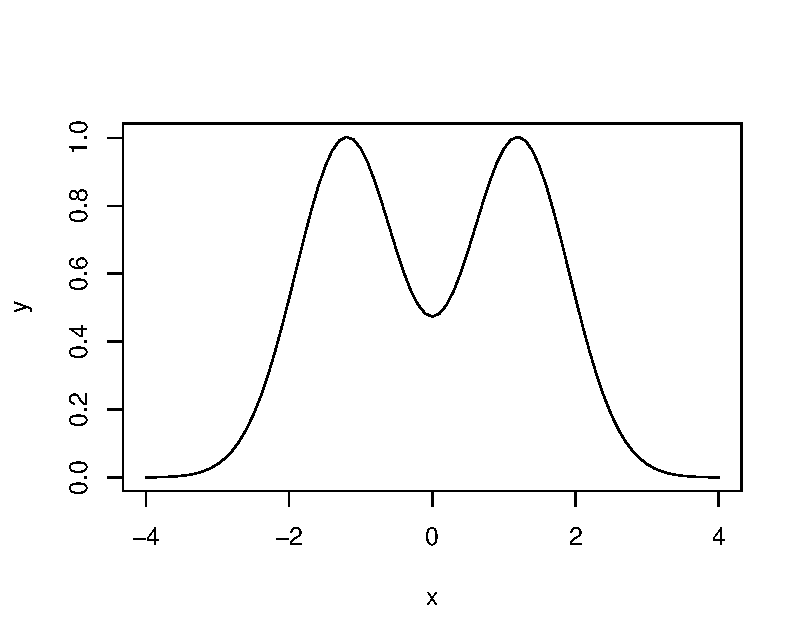
\includegraphics[width=0.3\tw]{fig/bimodal.pdf}
\end{center}

%===================================================================================
%===================================================================================
%===================================================================================
\section{Additional programs}
%===================================================================================
\subsection{Biner}\label{biner}
The program takes input track(s) and produces binned output track(s). Output tracks have bedGraph format. 
The name of the output is formed using the input name by adding binsize: \prm{<output>=<input\_fname>\_<binsize>}. The results will be written to the directory defined by \prm{binPath}.

Standard configuration file is \prm{stereogene.cfg}. Example of the configuration file:
\begin{shaded} 
\begin{verbatim}
chrom=chr_hg38.tab
trackPath=Tracks
binPath=Bin

bin=200
verbose=1
\end{verbatim}
\end{shaded}

\paragraph{Usage:}
\prm{\$ ./Binner <input\_fname>}\\
Standard batch conventions are used. User can use list files and directories
%===================================================================================
\subsection{Soother}\label{smoother}
The program takes a track and produces a smoothed track. The smoothing is done with given kernel (default -- Gaussian). 
$$
f_{smooth}(x)=\int f(t) \rho(x-t) dt
$$
The kernel width (smoothing width) defined by the \prm{kernelSigma} parameter. The resulting filename will have the suffix "\prm{\_sm}". The smoothed tracks are written to the directory \prm{smoothPath}. If the parameter \prm{smoothPath} is not defined, the results are written to \prm{trackPath}. 
To avoid boundary effects, the flanks are recommended for this program.
The default configuration file is \prm{stereogene.cfg}. Example configuration file:
\begin{shaded} 
\begin{verbatim}
chrom=chr_hg38.tab
trackPath=Tracks
smoothPath=Smooth

bin=200
wSize=1M
kernelSigma=10k
flankSize=50k
verbose=1
\end{verbatim}
\end{shaded}

\paragraph{Usage:}
\prm{\$ ./Smoother <input\_fname>}\\
Standard batch conventions are used. User can use list files and directories
%===================================================================================
\subsection{ParseGenes}\label{parseGenes}
It is often interesting to correlate some ChIP-seq data with gene features. To facilitate this comparison, the \prm{parseGenes} program parses the gtf file and produces 9 bed files:
\begin{center}
\begin{tabular}{ll}
Gene body&    \prm{<gtf\_file>\_gene.bed}   \\
Gene begins&  \prm{<gtf\_file>\_g\_beg.bed} \\
Gene ends&    \prm{<gtf\_file>\_g\_end.bed} \\
Exon body&    \prm{<gtf\_file>\_exn.bed}    \\
Exon begins&  \prm{<gtf\_file>\_e\_beg.bed} \\
Exon ends&    \prm{<gtf\_file>\_e\_end.bed} \\
Intron body&  \prm{<gtf\_file>\_ivs.bed}    \\
Intron begins&\prm{<gtf\_file>\_i\_beg.bed} \\
Intron ends&  \prm{<gtf\_file>\_i\_end.bed} \\
\end{tabular}
\end{center}


All this files will be written to the directory defined by the \prm{trackPath} parameter.
Program parameter \prm{gencodeLevel} defines the maximum confidence level of the GENECODE annotation (\url{https://www.gencodegenes.org/pages/data_format.html}) to be output by the program:
\begin{itemize}
\item 1 (verified loci),
\item 2 (manually annotated loci),
\item 3 (automatically annotated loci)
\end{itemize}
Program parameter \prm{biotypes} -- comma separated string of biotypes to be printed by the program. 
A complete list of biotypes can be found on the GENECODE web site \url{https://www.gencodegenes.org/pages/biotypes.html}. Example configuration file:
\begin{shaded} 
\begin{verbatim}
chrom=chr_hg38.tab
trackPath=Tracks

biotypes="lncRNA,lincRNA,protein_coding"
pgLevel=1
\end{verbatim}
\end{shaded}

\paragraph{Usage:}
\prm{\$ ./ParseGenes <input gtf file>}

%===================================================================================
%===================================================================================
\section{Make confounder}
\subsection{Program Confounder}
One of the possible confounders in histone modification analysis is nocleosome positioning. 
To find this confounder, we use the following algorithm. The program \prm{Confounder} takes the set of all available histone modification and creates a covariation matrix $Cov$.
Then the program searches for eigenvector $ev^{(1)}$ corresponding to the maximal eigenvalue.

Then, the confounder track is calculated as a linear combination of the tracks with the coefficients defined by the first eigenvector:
$$
cnf=\sum ev^{(1)}_i \cdot track_i
$$
Different tracks may have different scales. To eliminate such offsets, the tracks in this equation are normalized by the average value of the track.

The Confounder track is placed in the \prm{trackPath} directory. Its name is defined by the \prm{confounder} parameter. The default name is \prm{confounder.bgraph}. The program also creates a file \prm{confounder.covar} with the covariance matrix and the first eigenvector. This file is placed in the current working directory.

\paragraph{Usage:}
\prm{\$ ./Confounder <File\_list>}\\
where \prm{<File\_list>} -- list of the tracks or directory.

%===================================================================================
\subsection{Program Projector}
\sg can produce a projection orthogonal to the confounder.
But for batch analysis it seems to be more convenient to prepare a projection files in advance. 
Program \prm{Projector} makes such projections and creates a projection files. It adds new subdirectories \prm{<confounder\_name>.proj} to the \prm{Tracks}, \prm{Profiles} and \prm{Results} directories. Then the program creates projections and places them in appropriate directories. The program creates a new configuration file \prm{confounder.cfg} with modified parameters for directories and the parameter \prm{confounder} is removed.
\begin{tabular}{l|cr}
Old configuration && New configuration\\
\begin{minipage}{0.43\tw}
\begin{shaded} 
\begin{verbatim}
chrom=chr_hg38.tab
chrom=../chr_len_hg38.tab
trackPath=../Files/Tracks
profPath=../Files/profiles
resPath=../Files/res
report=report
confounder=confounder.bgraph

wSize=1M
bin=200
KernelSigma=30k
nShuffle=2000
maxNA=99.9
maxZero=99.9
localSuffle=1

plotType=pdf
crossWidth=30000
\end{verbatim}
\end{shaded}

\end{minipage}&&
\begin{minipage}{0.45\tw}
\begin{shaded} 
\begin{verbatim}
chrom=chr_hg38.tab
chrom=../chr_len_hg38.tab
trackPath=../Files/Tracks/confounder.proj/
profPath=../Files/profiles/confounder.proj/
resPath=../Files/res
report=report
#confounder=confounder.bgraph

wSize=1M
bin=200
KernelSigma=30k
nShuffle=2000
maxNA=99.9
maxZero=99.9
localSuffle=1

plotType=pdf
crossWidth=30000
\end{verbatim}
\end{shaded}
\end{minipage}
\end{tabular}
\paragraph{Usage:}
\prm{\$ ./Projector <File\_list>}\\
where \prm{<File\_list>} -- list of the tracks or directory.


\section{Comprehensive list of parameters}
%============================================================================================================
\newcommand{\hh}[1]{\\\hline\multicolumn{3}{c}{\textbf{#1}}}
\begin{longtable}{p{\cw}p{8cm}p{3cm}}

\caption{Full List of parameters} \label{paramList}\\\hline 

\hline \multicolumn{1}{|c|}{\textbf{Parameter}} & \multicolumn{1}{c|}{\textbf{Description}} & \multicolumn{1}{c|}{\textbf{Default value}} \\ \hline 
\endfirsthead

\multicolumn{3}{c}%
{{\bfseries \tablename\ \thetable{} -- continued from previous page}} \\
\hline \multicolumn{1}{|c|}{\textbf{Parameter}} & \multicolumn{1}{c|}{\textbf{Description}} & \multicolumn{1}{c|}{\textbf{Default value}} \\ \hline 
\endhead

\hline \multicolumn{3}{|r|}{{Continued on next page}} \\ \hline
\endfoot
\hline \hline
\endlastfoot


\hh{Paths}\\
\rcf{trackPath=<path>}
	&Path to the input tracks&
\rc{binPath=<path>}
	&Path to the output binned tracks (See section \ref{biner})&
\rc{smoothPath=<path>}
	&Path to the output smoothed tracks (See section \ref{smoother})&
\rc{profPath=<path>}
	&Path to profiles&
\rc{resPath=<path>}
	&Path to the result files&
\rc{report=<path>}
        &Path to the report files (pdf, html) relative to the resPath&
\hh{Files}
\rc{<fname>}
        &Input file. The name of the appropriate path is added  - trackPath. The Program can take up to 
        256 input files and calculate the correlation for every pair of the tracks. 
                &mandatory
\rc{chrom=<fname>}
        &Input file with names of chromosomes and their lengths (can ne downloaded from the Genome browser), 
        the parameter can be set in the config file or in the command line or as an environment variable SG\_CHROM. 
                &mandatory
\rc{cfg=<fname>}
        &Config file. It is possible to use more then one cfg-files. It is applied in order of appearance. 
        Parameters defined in the command line overrides the parameters in the config file.
        	&\prm{./stereogene.cfg}
\rc{confounder=<fname>}
        &The filename for confounder. The name is completed with  trackPath. For more details see Advanced features.
        The file can be produced by the 'confounder' program or defined by user. See Section \ref{confoud}&
\rc{statistics=<fname>}
        &File with the cumulative statistic for all the programm runs.
                & \prm{./statistics}
\rc{params=<fname>}
        &File for save the parameters for all the programm runs
                & \prm{./params}
\rc{aliases=<fname>}
        &File with aliases for brief track names. See Section \ref{aliases} &
\rc{log=<fname>}
        &Log-file name. To toggle log output OFF use empty name for the log file. If the user starts the 
        log-file name with '\$' the '\$' character will be replaced by the current output filename. 
                & \prm{./stereogene.log }\\
\hh{General}                
\rc{verbose=<ON|OFF>}
        &The program workflow is printed to standard output
                &\prm{OFF}
\rc{-v}
        &Is used for command line only. Equivalent to verbose=ON&
\rc{silent=<ON|OFF>}
        &If ON the general results are not printed to stdout.
                &\prm{OFF}
\rc{-s}
        &Is used for command line only. Equivalent to silent=ON&
\rc{syntax=<ON|OFF>}
        &If this flag is set ON the program will terminate with error on wrong line in input profile; 
        the line will be ignored otherwise
                &\prm{ON}
\rc{-syntax}
        &Is used for command line only. Equivalent to syntax=OFF&
\rc{BufSize}
        &Size of the buffer in swap-file-arrays&100000000
\hh{Preprocessing}
\rc{clear=<0 | 1>}
        &Force profile preprocessing
                &0
\rc{-c}
        &Is used in command line only. Is equal to clear=1 &
\rc{bin = <num>}
        &bin for sliding frame. Optional. 
                &100
\rc{bpType=< SCORE |\newline SIGNAL | LOGPVAL >}
        &The value used as a score for BroadPeak format -- column Score, Signal, or pval
                &\prm{SCORE}
\hh{Correlation}
\rc{wSize=<num>}
	&Window size (in nucleotides)
		&100000
\rc{wStep=<num>}
        &Window step (in nucleotides)
                &100000
\rc{kernelType=< NORMAL | LEFT\_EXP | RIGHT\_EXP >}
        &       Kernel type: \newline
        NORMAL    -- Normal\newline
        LEFT\_EXP  -- left exponent\newline 
        RIGHT\_EXP -- right exponent    
                &\prm{NORMAL}    
\rc{customKern = <expression>}
        &An expression that defines the kernel function. See the section Section \ref{custKernel}. 
        If  the custom kernel defined the prameter kernelType will be ignored.&
\rc{KernelSigma=<num>}
        &Kernel span (in nucleotides)
                &1000
\rc{kernelShift=<num>}
        &Kernel mean (for Gauss) or Kernel start for exponent
                &0
\rc{kernelNS=<num>}
        &Inhibit Zero position of the kernel. The kernel values in the interval [-100,100] will be 
        multiplied by (1- kernelNS)
                &0
\rc{complFg=< COLLINEAR | COMPLEMENT | IGNORE\_STRAND>}
        &       Flag: \newline
        IGNORE\_STRAND -- ignore strand;\newline
        COLLINEAR -- compare collinear strands; \newline
        COMPLEMENT -- compare opposed strands. \newline
        If the binary profiles are not separated by strand that works in IGNORE\_STRAND         
        	&\prm{IGNORE\_STRAND}
\rc{NA=<0 | 1>}
        &The way to treat uncertain values. If flag is 0, then uncertain (not covered with profile) values 
        are considered as 0. Otherwise it is filled by a random noise (see noiseLevel parameter). 
        This flag has no sense for BED tracks. For this type the flag is ignored and  uncertain values are 
        considered as 0.
                &0
\rc{-na}
        &Is used in command line only. Is equal to NA=1 &
        
\rc{flankSize=<num>}
        &Size of added flanks (in nucleotides). Nesessary to avoid side effects. Recommended value\newline
         $2\cdot KernelSigma $
                &0
\rc{noiseLevel=<num>}
        &Noise level used to fill flanks and uncertain values. The uncertain values is defined as 
        $rExp()\cdot sd\cdot noiseLevel$, where  rExp() -- standard exponential random value, 
        sd -- standard deviation of track values.
                &0.2
\rc{maxNA=<num>}
        &Maximum fraction of uncertain values  in a frame (percent). If at least one of the compared frames has maxNA 
        (or more) of uncertain values, then the comparison is not applied. 
                &99
\rc{maxZero=<num>}
        &Maximum fraction of zero values  in a frame (percent). If at least one of the compared frames has maxZero 
        (or more) of zero values, then the comparison is not applied.  If parameter the takes 100, it is possible 
        to get false peak for correlation value 1. 
                &99
\rc{nShuffle=<num>}
        &Number of permutations to build the background distribution. 
                &10000
\rc{threshold=<num>}
        &The threshold values for the binary profile. If the binary value is less than the threshold profile, 
        it is replaced by 0. 0 < threshold < 256
                &0
\rc{localShuffle}
        &Use cyclic window shuffle
                &1    
                
\hh{Output definition parameters}
\rc{outRes=< XML | TAB | BOTH | NONE>}
        &Output cumulative result and parameters: \newline
        XML -- output in xml-like format\newline
        TAB -- output in tabbed form\newline
        BOTH -- output in both format\newline
        NONE -- not output cumulative information
                &\prm{BOTH}
\rc{outPrjBGr=<0|1>}
        &Flag: write bed-graph files for Projections.
                &1
\rc{outDistr=<0|1>}
        &Flag: write foreground and background distributions into files \prm{<track1>$\sim$<track2>.fg, <track1>$\sim$<track2>.bkg}
                &1
\rc{aliases=<file>}
        & Filename with rules for replacing track names in output filenames (see section \ref{aliases})
                &
\rc{outChrom=<0|1>}
        &Write statistics by chromosomes (file \prm{<track1>$\sim$<track2>.chrom})
                &0
\rc{Cross=<0|1>}
        &Flag: write Distance correlations (file \prm{<track1>$\sim$<track2>.dist})
        If the parameter outChrom is ON the distance information will be given by chromosomes.
                &1
\rc{WriteDistr=<NONE | SHORT | DETAIL>}
        &Write the Foreground and Background correlation distributions. If the value set to  'DETAIL' the positional 
                information for foreground will be written.
        &\prm{SHORT}
\rc{outSpectr=<0|1>}
        &Write average spectrum. File \prm{<track1>$\sim$<track2>.spect}
                &0
\rc{AutoCorr=<0 | 1 >}
        &Write autocorrelation. The autocorrelation function is written to a file Track.auto. 
        If  lAauto = 0, 
        the autocorrelation is not considered.
                &0
\rc{plotType=<NONE | R |PDF | HTML | ALL>}
        &
        Write the script to the R to plot the results. The name of the script file is generated from the
         output file name.      Values mean:\newline
                R -- R script for just plotting\newline
                PDF -- R script for producing pdf file\newline
                HTML -- R script for producing HTML report
                &0
\rc{-r}
        &Is used in command line only. Equals to plotType=R&
\rc{crossWidth}
        &Define width for cross-correlation plots
                &10000
\rc{Rscript}
        &Command to run R script. If the parameter defined the program will call R automatically.
                &Rscript
\rc{plotW}
        &Plot width     &4
\rc{plotH}
        &Plot height
                &3
\rc{OutLC=<0 | BASE | CAENTER>}
        & Flag: Write local kerneled correlations into a bedgraph file.
        & 0
\rc{-lc}
        &Is used in command line only. Equals to outLC=BASE&
\rc{LCScale=<LIN|LOG>}
        & 
        Scaling for the Local Correlation output: \newline
        LIN     -- Use linear scaling to the interval (0..1000)\newline
        LOG     -- Use logarithmic scaling:\newline
        $v = sign(w)*\log(1+|w|)$           
                &\prm{LOG}
\rc{L\_LC = <num>}
        &Threshold for local kernel correlation  for low (usually negative) local correlations to be written 
        into the local correlation file:  $corr \leq L\_LC$ will be written. 
        &-20
\rc{R\_LC = <num>}
        &Threshold for local kernel correlation for high local correlations to be written into the 
        local correlation file:  $corr \geq R\_LC$ will be written. 
                &1
\rc{gencodeLevel=<1|2|3>}
        &Maximal confidence level in the GENCODE gtf file. See section \ref{parseGenes} 
                &2
\rc{biotypes= <string>}
        &list of biotypes to be printed by ParseGenes program. See section \ref{parseGenes} 
                &
                
\\\hline
\end{longtable}


%===================================================================================
%===================================================================================
%===================================================================================
\section{Output file formats}\label{fmt}
%===================================================================================
\subsection{Background correlations \prm{<track1>$\sim$<track2>.bkg}}

\prm{<track1>$\sim$<track2>.bkg} -- Array  of correlations of shuffled windows

\begin{minipage}{0.2\tw}
\begin{shaded} 
\begin{verbatim}
 0.320268
 0.178365
-0.419948
-0.124017
 0.298771
   ...
\end{verbatim}
\end{shaded}
\end{minipage}

%============================================================================================================
%============================================================================================================
\subsection{Correlations in coherent windows \prm{<track1>$\sim$<track2>.fg}}
Output depends on the parameter \prm{writeDistr}. 

%============================================================================================================
\subsubsection{Short format (\prm{writeDistr=SHORT)}}
 
\begin{minipage}{0.2\tw}
\begin{shaded} 
\begin{verbatim}
 0.320268
 0.178365
-0.419948
-0.124017
 0.298771
   ...
\end{verbatim}
\end{shaded}
\end{minipage}

%============================================================================================================
\subsubsection{Detailed Format (\prm{writeDistr=DETAIL)}}

\begin{minipage}{0.5\tw}
\begin{shaded} 
\begin{verbatim}
chr1     7500000       7500100    -0.093813
chr1     7750000       7750100    -0.531958
chr1     8000000       8000100    -0.425593
chr1     8250000       8250100    -0.479256
chr1     9750000       9750100    -0.466759
...                              
\end{verbatim}
\end{shaded}
\end{minipage}

\paragraph{columns:} Chromosome, window start,  window end, correlation

%============================================================================================================
%============================================================================================================
\subsection{Distances distribution (correlation function) \prm{<track1>$\sim$<track2>.dist}}
\prm{<track1>$\sim$<track2>.dist} – Distances distribution (cross-correlation function) for background, foreground, chromosomes.
Output depends on the parameter \prm{outChrom}. 
%============================================================================================================
\subsubsection{Sort format (\prm{outChrom=0)}}

\paragraph{Contains:}
\begin{tabular}{ll}
dist   & -- Distance (nucl)\\
Bkg    & -- background cross-correlation function\\
Fg     & -- foreground cross-correlation  function\\
FgPlus & -- cross-correlation  function for windows with positive correlations\\
FgMinus& -- cross-correlation  function for windows with negative correlations
\end{tabular}

\paragraph{Example:}\;\;
\begin{minipage}{0.6\tw}
\begin{shaded} 
\begin{verbatim}
# Track1 vs Track2
dist       Bkg        Fg        FgPlus     FgMinus
-500000  -0.04668   -0.91321   -1.13892    0.42649
-499800	 -0.03251   -0.90076   -1.11362    0.36262
-499600	 -0.06510   -0.87523   -1.07763    0.32609
                   ...  
499400   -0.06324   -0.89405   -1.10051    0.33138
499600   -0.04718   -0.89841   -1.10964	   0.35531
499800   -0.05677   -0.90264   -1.12193	   0.39892                            
\end{verbatim}
\end{shaded}
\end{minipage}

%============================================================================================================
\subsubsection{Full format (\prm{outChrom=1)}}
In this case the file \prm{<track1>$\sim$<track2>.dist} will have additional information by chromosomes.

\paragraph{Example:}\;\;
\begin{minipage}{0.85\tw}
\begin{shaded} 
\begin{verbatim}
# SMARCA5_100 vs SMARCB1_100
 dist       Bkg         Fg          FgPlus      FgMinus     chr1      chr2    ...
-500000    -0.02757    -1.60256    -1.69173     0.07157    -1.418    -1.217   ...
-499800    -0.01842    -1.57518    -1.66986     0.20262    -1.392    -1.208   ...
                    ...
 499600    -0.01402    -1.58403    -1.68101     0.23669    -1.389    -1.223   ...
 499800    -0.02548    -1.60363    -1.69075     0.03198    -1.422    -1.210   ...
\end{verbatim}
\end{shaded}
\end{minipage}
%============================================================================================================
%============================================================================================================
\subsection{Local correlation track}\label{LC}

\prm{<track1>$\sim$<track2>.bgraph} -- a bed graph file for kerneled local correlations. This track can be used for kerneled correlation visualization with Genome Browser. The track can also be used for further analysis, such as peak calling and searching the correlation of this track with other tracks. 
Note, The values can be positive or negative and can be outside the interval [-1,1].


This output regulates by \prm{outLC} parameter. This parameter can take 3 possible values:

\begin{tabular}{ll}\\
0	         & -- No local correlation produced\\
\prm{BASE}   & -- The local correlation will be based on zero. No negative values will be produced\\
\prm{CENTER} & -- The local correlation will be based on mean. Negative values will be produced\\ \\
\end{tabular}

The program also used 2 additional parameters for filter the output:

\begin{tabular}{ll}\\
\prm{L\_LC} & -- Threshold for local kernel correlation  for low (usually negative) local correlations to be written 
        into the local correlation file:  $corr \leq L\_LC$ will be written. \\
\prm{R\_LC} & -- Threshold for local kernel correlation for high local correlations to be written into the 
        local correlation file:  $corr \geq R\_LC$ will be written. \\ \\
\end{tabular}

Format: Standard graph format (see Genome Browser documentation). The file may contain a comment line defining segments without data. These segments appear if the source tracks do not contain any data here.
 
\begin{minipage}{0.75\tw}
\begin{shaded} 
\begin{verbatim}
track type=bedGraph name="track1~track2" description="Local correlation"
#chr1	0	860800	?
chr1	861100	861600	1.5
chr1	861600	861700	1.4
        ...
\end{verbatim}
\end{shaded}
\end{minipage}

If the parameter \prm{writeDistr=DETAILS} the file \prm{<track1>$\sim$<track2>.LChist} is also written.  This file contains the statistical information of the local correlations. 
The file represents a histogram and contains the following columns

\begin{tabular}{ll}
\prm{corr} & local correlation\\
\prm{obs} 			& observed density \\
\prm{nObs} & number of observations\\
\prm{exp } & Expected density\\
\prm{nExp} & number of observations in the background\\
\prm{r\_CDF\_obs} & $1-cdf(corr)$ for observed values\\
\prm{r\_CDF\_exp} & $1-cdf(corr)$ for the background\\
\prm{R\_FDR} & FDR for value less than corr (percent)\\
\prm{l\_CDF\_obs} & $cdf(corr)$ for observed values\\
\prm{l\_CDF\_exp} & $cdf(corr)$ for the background\\
\prm{L\_FDR} & FDR for value to be greater than corr (percent)\\
\end{tabular}
\begin{shaded} 
\begin{scriptsize}
\begin{tabular}{lllllllllll}
corr&obs&nObs&exp&nExp&r\_CDF\_obs&r\_CDF\_exp&R\_FDR&l\_CDF\_obs&l\_CDF\_exp&L\_FDR\\
0.01&3.58E+001&14530762&1.48E+000&602387&1.00E+000&1.00E+000&100&1.00E+000&4.14E-002&4.15\\
0.04&1.06E-004&43&1.62E-001&65825&2.92E-004&9.59E-001&100&1.00E+000&4.60E-002&4.6\\
0.07&6.40E-005&26&1.54E-001&62385&2.89E-004&9.54E-001&100&1.00E+000&5.03E-002&5.03\\
0.1&4.68E-005&19&1.31E-001&53067&2.87E-004&9.50E-001&100&1.00E+000&5.39E-002&5.39\\
&&...&&&...&&&...&&\\
1.64&7.39E-006&3&1.02E-003&415&2.68E-004&6.67E-005&24.85&1.00E+000&1.00E+000&100\\
1.66&4.92E-006&2&9.31E-004&378&2.68E-004&3.81E-005&14.22&1.00E+000&1.00E+000&100\\
1.69&9.85E-006&4&4.33E-004&176&2.68E-004&1.21E-005&4.52&1.00E+000&1.00E+000&100\\
1.72&4.92E-006&2&0.00E+000&0&2.68E-004&0.00E+000&0&1.00E+000&1.00E+000&100\\
1.75&7.39E-006&3&0.00E+000&0&2.68E-004&0.00E+000&0&1.00E+000&1.00E+000&100\\
&&...&&&...&&&...&&\\
12.53&1.13E-004&46&0.00E+000&0&1.09E-005&0.00E+000&0&1.00E+000&1.00E+000&100\\
12.56&2.56E-004&104&0.00E+000&0&7.77E-006&0.00E+000&0&1.00E+000&1.00E+000&100\\
12.59&2.22E-005&9&0.00E+000&0&6.19E-007&0.00E+000&0&1.00E+000&1.00E+000&100\\
\end{tabular}
\end{scriptsize}
\end{shaded}

\subsection{Autocorrelation \prm{track.auto}}
When the parameter \prm{AutoCorr=1} the autocorrelation for tracks will be written:

\paragraph{Example:}\;\;
\begin{minipage}{0.25\tw}
\begin{shaded} 
\begin{verbatim}
-500000   -0.01006
-499800   -0.01045
      ...
   -200    0.20834
      0    1.00000
    200    0.20834
       ...
 499600   -0.00998
 499800   -0.01045 
\end{verbatim}
\end{shaded}
\end{minipage}

\subsection{Spectrum density}
When the parameter \prm{outSpectr=1} the spectrum for tracks will be written to the file \prm{<track1>$\sim$<track2>.spect}:

\paragraph{Example:}\;\;
\begin{minipage}{0.35\tw}
\begin{shaded} 
\begin{verbatim}
#	Track1	Track2
Wave_Length  Spectrum1  Spectrum2
1000000.00     6.277      2.053
 500000.00     6.234      2.042
 ...
\end{verbatim}
\end{shaded}
\end{minipage}

\subsection{Chromosome statistics \prm{<track1>$\sim$<track2>.chrom}}
The file contains:
\begin{tabular}{ll}
Chrom    & Chromosome name\\
av1      & Average signal in track1\\
av2      & Average signal in track2\\
cc       & Average correlation\\
count    & Number of non-zero windows\\
\end{tabular}

\paragraph{Example:}\;\;
\begin{minipage}{0.35\tw}
\begin{shaded} 
\begin{verbatim}
Track1
Track2
 chrom	  av1 	  av2 	  cc 	count
  chr1  758.94  611.39   0.58   232
  chr2  660.22  562.58   0.61   242
  chr3  640.48  558.50   0.60   197
\end{verbatim}
\end{shaded}
\end{minipage}

\section{Statistics.tsv – total statistics for all runs}
This is a cumulative file with results. The file name can be changed using parameter \prm{statistics}.

The file contains a table with columns:

\begin{tabular}{ll}
\prm{id }         &  Run ID          \\
\prm{Date }       &  Date/Time of the end of the run in format:    13.05.17 15:13:59           \\
\prm{version}     &  Program version           \\
\prm{name1}       &  Name of the first track           \\
\prm{name2}       &  Name of the second track            \\
\prm{nFgr }       &  Number of foreground observations           \\
\prm{nBkg }       &  Number of background observations           \\
\prm{Fg.Corr}     &  Average correlation for coherent windows           \\
\prm{FgCorr\_sd}  &  Standard deviation of the correlation for coherent windows           \\
\prm{Bg.Corr}     &  Average correlation for shuffled windows           \\
\prm{BgCorr\_sd}  &  Standard deviation of the correlation for shuffled windows           \\
\prm{Mann-Z }     &  Man-Whitney Z-score            \\
\prm{p-value}     &  Man-Whitney p-value           \\
\prm{PDF\_report} &  Filename of the pdf report           \\
\prm{HTML\_report}&  Filename of the html report           \\
\prm{kernelSigma} &  Kernel Width           \\
\prm{wSize}       &  Window size           \\
\end{tabular}

Example:

\begin{minipage}{0.95\tw}
\begin{shaded}
\begin{scriptsize}
\begin{tabular}{llllllllll}
id       & Date              & version & name1       & name2       & nFgr & nBkg & Fg. Corr & FgCorr\_sd & Bg. Corr\\
6578d779 & 25.07.24 19:51:16 & 2.44    & SMARCA5\_100 & SMARCB1\_100 & 2907 & 2907 & 0.606    & 0.300    & 0.0122  \\
6580808f & 25.07.24 19:59:38 & 2.44    & SMARCA5\_100 & SMARCB1\_100 & 2907 & 2907 & 0.606    & 0.300    & 0.0122  \\
\end{tabular}
\end{scriptsize}
\end{shaded}
\end{minipage} 

Continue of the table


\begin{flushright}
\begin{minipage}{0.85\tw}
\begin{shaded} 
\begin{scriptsize}
\begin{tabular}{lllllll}
 BgCorr\_sd & Mann-Z & p-value  & PDF\_report                   & HTML\_report & kernelSigma & wSize  \\
 0.375      & 50.412 & 0.00e+00 & SMARCA5\_100$\sim$SMARCB1\_100.pdf &              & 30000       & 1000000\\
 0.375      & 50.412 & 0.00e+00 &                               &              & 30000       & 1000000\\
\end{tabular}
\end{scriptsize}
\end{shaded}
\end{minipage} 

\end{flushright}


\subsection{File Parameters.tsv}
This file contains all the parameters (including the default values) for the \sg run. 
The correspondence of rows in this table with \prm{Statistics.tsv} can be determined by the run id.

\begin{flushleft}
\begin{minipage}{0.9\tw}
\begin{shaded} 
\begin{scriptsize}
\begin{tabular}{llllllllll}
id       & version & bin & profPath           & trackPath        & resPath       & report  & chrom             & bpType& NA \\
6578d779 & 2.50    & 200 & ../Files/profiles/ & ../Files/Tracks/ & ../Files/res/ & report/ & chr\_len\_hg38.tab& SIGNAL& 0  \\
6580808f & 2.50    & 200 & ../Files/profiles/ & ../Files/Tracks/ & ../Files/res/ & report/ & chr\_len\_hg38.tab& SIGNAL& 0  \\
\end{tabular}
\end{scriptsize}
\end{shaded}
\end{minipage}
\end{flushleft}
Continue of the table
                                                                                                                        \begin{flushright}                                                                                                                        \begin{minipage}{0.9\tw}
\begin{shaded} 
\begin{scriptsize}
\begin{tabular}{llllllllll}
 threshold & kernelType & customKern & kernelSigma & kernelShift & wSize   & wStep   & flankSize & maxNA & maxZero\\
 0         & NORMAL     & NONE       & 30000       & 0           & 1000000 & 1000000 & 0         & 1e+02 & 1e+02  \\
 0         & NORMAL     & NONE       & 30000       & 0           & 1000000 & 1000000 & 0         & 1e+02 & 1e+02  \\
\end{tabular}
\end{scriptsize}
\end{shaded}
\end{minipage}                                                                                                                         \end{flushright}

Continue of the table

\begin{flushright}
\begin{minipage}{0.9\tw}
\begin{shaded} 
\begin{scriptsize}
\begin{tabular}{llllllllllll}
 nShuffle & noiseLevel & complFg & localSuffle & outSpectr & outChrom & writeDistr & plotType & Cross & outLC & L\_LC \\
 2000     & 0          & IGNORE\_ & 1           & 0         & 1        & DETAIL     & PDF     & 1     & NA    & -20   \\
 2000     & 0          & IGNORE\_ & 1           & 0         & 1        & DETAIL     & PDF     & 1     & NA    & -20   \\
\end{tabular}
\end{scriptsize}
\end{shaded}
\end{minipage} 
\end{flushright}

Continue of the table

\begin{flushright}
\begin{minipage}{0.7\tw}
\begin{shaded} 
\begin{scriptsize}
\begin{tabular}{llllll}
 R\_LC &AutoCorr & aliases & Rscript                                        & plotH &plotW\\
 1     &0        & aliases & C:/Program Files/R/R-3.6.0/bin/x64/Rscript.exe & 3     & 7   \\ 
 1     &0        & aliases & C:/Program Files/R/R-3.6.0/bin/x64/Rscript.exe & 3     & 7   \\
\end{tabular}
\end{scriptsize}
\end{shaded}
\end{minipage} 

\end{flushright}





\end{document}
%============================================================================================================
%============================================================================================================
%============================================================================================================
%============================================================================================================
%==============================================================================================================
%==============================================================================================================
%==============================================================================================================
%==============================================================================================================
%==============================================================================================================
